%%%%%%%%%%%%%%%%%%%%%%%%%%%%%%%%%%%%%%%%%
% a0poster Portrait Poster
% LaTeX Template
% Version 1.0 (22/06/13)
%
% The a0poster class was created by:
% Gerlinde Kettl and Matthias Weiser (tex@kettl.de)
% 
% This template has been downloaded from:
% http://www.LaTeXTemplates.com
%
% License:
% CC BY-NC-SA 3.0 (http://creativecommons.org/licenses/by-nc-sa/3.0/)
%
%%%%%%%%%%%%%%%%%%%%%%%%%%%%%%%%%%%%%%%%%

%----------------------------------------------------------------------------------------
%	PACKAGES AND OTHER DOCUMENT CONFIGURATIONS
%----------------------------------------------------------------------------------------

\documentclass[a0,portrait]{a0poster}

\usepackage{multicol} % This is so we can have multiple columns of text side-by-side
\columnsep=100pt % This is the amount of white space between the columns in the poster
\columnseprule=3pt % This is the thickness of the black line between the columns in the poster

\usepackage[svgnames]{xcolor} % Specify colors by their 'svgnames', for a full list of all colors available see here: http://www.latextemplates.com/svgnames-colors

\usepackage{times} % Use the times font
%\usepackage{palatino} % Uncomment to use the Palatino font

\usepackage{graphicx} % Required for including images
\graphicspath{{figures/}} % Location of the graphics files
\usepackage{booktabs} % Top and bottom rules for table
\usepackage[font=small,labelfont=bf]{caption} % Required for specifying captions to tables and figures
\usepackage{amsfonts, amsmath, amsthm, amssymb} % For math fonts, symbols and environments
\usepackage{wrapfig} % Allows wrapping text around tables and figures
\usepackage[utf8]{inputenc}
\usepackage{cite}

\begin{document}

%----------------------------------------------------------------------------------------
%	POSTER HEADER 
%----------------------------------------------------------------------------------------

% The header is divided into two boxes:
% The first is 75% wide and houses the title, subtitle, names, university/organization and contact information
% The second is 25% wide and houses a logo for your university/organization or a photo of you
% The widths of these boxes can be easily edited to accommodate your content as you see fit

\begin{minipage}[b]{0.75\linewidth}
\veryHuge \color{NavyBlue} \textbf{Proposta de um Modelo para Comportamentos Não-Normativos } \color{Black}\\ % Title
\huge \textbf{Jonathan Morris Samara, Cesar Augusto Tacla}\\[0.5cm] % Author(s)
\huge Institutos Lactec, Copel,UFPR,UTFPR - Projeto RV2\\[0.4cm] % University/organization
\Large \texttt{jonathan.samara@lactec.org.br} 
\end{minipage}
%
\vspace{1cm} % A bit of extra whitespace between the header and poster content

%----------------------------------------------------------------------------------------

\begin{multicols}{2} % This is how many columns your poster will be broken into, a portrait poster is generally split into 2 columns

%----------------------------------------------------------------------------------------
%	ABSTRACT
%----------------------------------------------------------------------------------------

\color{Navy} % Navy color for the abstract

\begin{abstract}

\end{abstract}

%----------------------------------------------------------------------------------------
%	INTRODUCTION
%----------------------------------------------------------------------------------------

\color{SaddleBrown} % SaddleBrown color for the introduction

\section*{Introdução}

A comunidade acadêmica atual apresenta grande preocupação no que tange a criar modelos lógicos
com propósito de representar o comportamento de organizações humanas. Neste aspecto, há uma 
especial preocupação em modelar comportamentos normativos e suas respectivas violações.
Estudos de comportamentos não-normativos fazem uso de lógica deontica para definir obrigações e 
e permissões. Esses estudos modelam uma violação como o não cumprimento de uma determinada norma. 
A violação de uma determinada norma implica uma sanção (penalidade sobre a qual o agente está sujeito)
\cite{SimulationNonNormative},\cite{ControllingNonNormative}.

Os modelos atuais apresentam representações adequadas para violações cujas sanções são imediatas a 
violação. Alguns modelos levam em consideração realidades onde determiandas violações podem ou não 
ocasionar sanções \cite{HowDoAgentMakeDecision}. Contudo, esses modelos não levam em consideração
como uma determinada violação gera consequências em objetivos futuros. 
		  
Diversas atividades do cotidiano se enquadram na situação onde uma violação não gera consequências
imediatas, contudo ocasionam problemas futuros. Para exemplicar é possível imaginar uma situação
onde um técnico deve se deslocar do ponto A até o ponto B para realizar uma determinada manutenção
corretiva no ponto B. Para isso, o técncio deve levar consigo a ferramenta f1 que está no ponto A. 
Assim sendo, esse caso pode ser modelado por meio de uma abordagem normativa onde o técnico é
obrigado a pegar a ferramenta f1 do ponto A, é obrigado a levar consigo do ponto A até o ponto B e
é obrigado a usar a ferramenta no ponto B. Se o técnico esquecer de pegar a ferramenta no ponto A,
ele comete uma violação. Contudo, nenhuma sanção imediata ocorre sobre ele. Não apenas isso, certas
atividades não são impedidas de acontecer. Contudo, o técnico não conseguirá executar a obrigação de 
usar a ferramenta no ponto B tendo em vista sua respectiva violação. Assim sendo, há interesse 
científico em criar modelos para representar esse tipo de situação.

%----------------------------------------------------------------------------------------
%	OBJECTIVES
%----------------------------------------------------------------------------------------

\color{} % DarkSlateGray color for the rest of the content

\section*{Objetivos Principais}

O objetivo geral deste estudo implica propor um modelo para representar consequências indiretas em 
objetivos futuros que podem acontecer dada ocorrência de uma determianda violação. Esse modelo 
será usado para descrever um estudo de caso onde eletricistas praticam manutenção em linha viva.
Uma manutenção em linha viva é um tipo de manutenção que ocorre sobre equipamentos elétricos de alta-tensão 
onde os mesmos se mantêm energizados. 

\begin{enumerate}
\item Verificar modelos e conceitos que podem ser utilizados no modelo proposto por esse estudo.
\item Verificar adaptações de modelos para este estudo em específico.
\item Criar conceitos e relações necessários ao propósito do modelo. 
\item Especificar o estudo de caso no modelo proposto.
\item Implementar o modelo em uma linguagem de programação.
\end{enumerate}



%----------------------------------------------------------------------------------------
%	MATERIALS AND METHODS
%----------------------------------------------------------------------------------------

\section*{Metodologia}

A primeira etapa metodológica desta pesquisa consistiu em identificar modelos que podem ser
usados para a finalidade deste estudo. Os pesquisadores identificaram um modelo em específico 
denominado de MOISE+\cite{AutonomousAgent}. O MOISE visa especificar o comportamento de um 
\textit{MAS} - Sociedade Multi-Agente. O MOISE+ leva em consideração que cada agente deve ter
um papel. Esse papel está vinculado a uma determianda missão. Está, por sua vez, engloba 
uma série de objetivos. O MOISE+ também leva em consideração questões organizacionais envolvendo
grupos, links e compatibilidades entre papeis. Este modelo apresenta relações de obrigação,
contudo não define relações de violação para as obrigações. Para a tratativa de vioalação de uma
norma, foi feito uso dos conceitos presentes no estudo \cite{ControllingNonNormative}.

A segunda etapa metodologica desta pesquisa consistiu em analisar o caso de estudo (manutenção em linha viva).
Para isso os pesquisadores analisaram procedimentos de manutenção sendo postos em prática, analsiaram 
documentos técnicos, entrevistaram engenheiros especialistas na área. 

A terceira etapa metodologia se deu por criar conceitos, criar relaçoes, adaptar conceitos de outros modelos, 
definri relaçoes dos conceitos novos com os conceitos de outros modelos e verificar como este modelo resultante
se adapta ao estudo de caso.

A quarta etapa metodologica consistiu usar todos o material desenvolvido na terceira etapa na criação 
de um UML.

A quinta etapa metodologica se deu por implementar o modelo em Prolog (linguagem de programação). Para isso
o modelo foi escrito em relacionamentos de predicados. Uma vez feito isso, os pesquisadores realizaram diversas
consultas e inferências a fim de identificar relações de interesse a pesquisa. 

A sexta etapa consistiu em verificar se o modelo estava de acordo com o esperada tanto em relação a realidade 
como em relação aos seus propósitos.

\section*{Resultados}

A figura \ref{figUmModelSimulation} apresenta uma representação em UML do modelo resultante. A figura estrutura em 
quatro blocos principais. O bloco \textit{MaintenanceAspects} apresenta todos os aspectos vinculados a manutenção 
propriamente dita, o bloco \textit{SanctionCondition} apresenta as sansações que ocorrem na violação de uma norma,o 
bloco \textit{MOISE+} consiste em uma representação similar ao modelo \textit{MOISE+} e o bloco \textit{SafetyEngineering}
apresenta todos os possíveis riscos com base em critérios de engenharia de segurança.

\begin{center}\vspace{1cm} 
	\label{figUmlModelSimulation}
	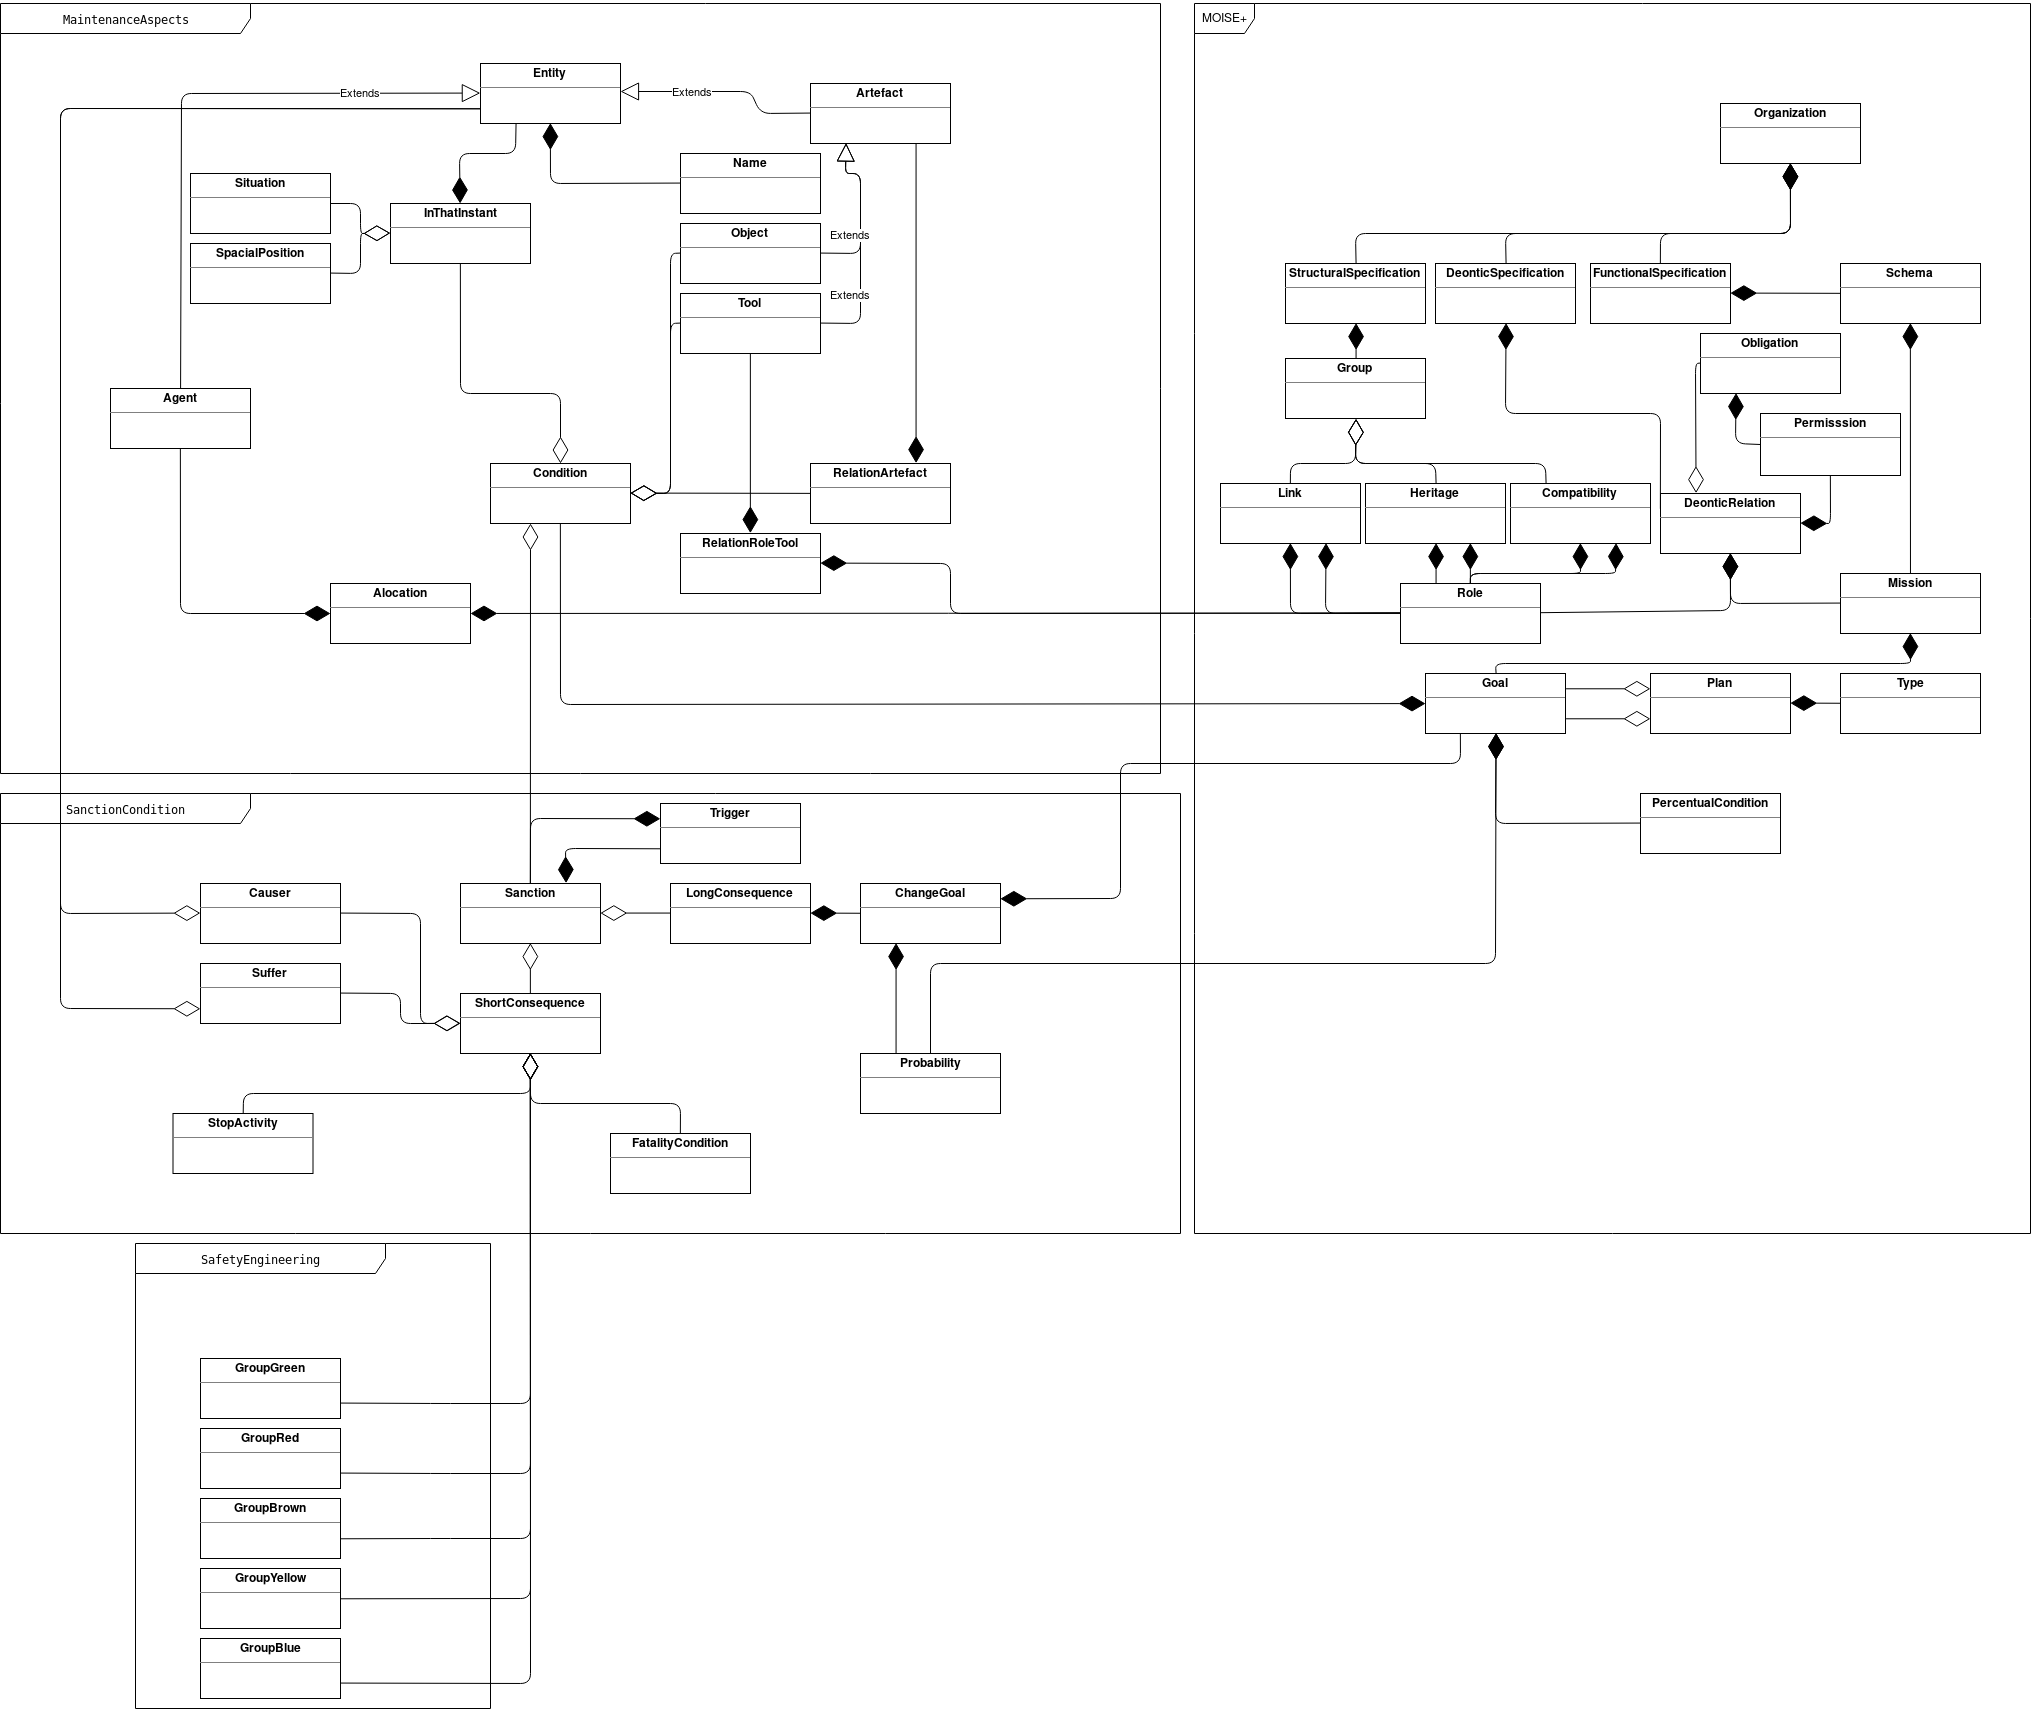
\includegraphics[width=1\linewidth]{uml_model_simulation}
	\captionof{figure}{\color{Green} Modelo resultante deste estudo escrito em UML}
\end{center}\vspace{1cm} 



Inspirado no \textit{MOISE+}, este modelo define uma relação deontica de obrigatoriedade com base na missão e no papel. 
Contudo, também assume como verdade a seguinte relação. 

\begin{equation}\label{deontilogic}
	obligation(\rho,mission)\wedge hasGoal(mission,goal) \to obligation(\rho,goal)
\end{equation}

A relação na implicabilidade \ref{deontilogic} tem que ser assumida como verdadeira, pois uma sanção é especificada em 
relação ao objetivo propriamente dito. Assim sendo, com base no modelo pode-se chegar a relação \ref{sanction}

\begin{equation}\label{sanction}
	\sim obligation(\rho,goal) \to sanction(\rho,goal,name_{sanction})
\end{equation}

\begin{equation}\label{lconsequence}
	sanction(\rho,goal) \to longConsequence(goal_{b}) 
\end{equation}

\begin{equation}\label{lconsequencen1}
	longConsequence(goal) \wedge hasProbability(goal,probability) \to hasProbability(goal,newProbability)
\end{equation}
\begin{equation}\label{lconsequencen2}
	 hasProbability(goal,newProbability)\to (newProbability < probability)
\end{equation}
\begin{equation}\label{risk}
	sanction(\rho,goal,name_{sanction}) \to exist(risk,\rho) 
\end{equation}
\begin{equation}\label{sanctionTrigger}
		  trigger(name_{sanction-start},name_{sanction-fire}) \to happens(name_{sanction-start})
\end{equation}
\begin{equation}\label{sanctionTrigger02}
		  trigger(name_{sanction-start},reason) \to happens(name_{sanction-start})
\end{equation}


----------------------------------------------------------------------------------------
\bibliographystyle{plain} % Plain referencing style
\bibliography{sample} % Use the example bibliography file sample.bib

\end{multicols}
\end{document}
